

%build with
%pdflatex main.tex 2>&/dev/null ; bibtex main 2>&/dev/null ; latexmk -pdf -f -g -bibtex -deps -synctex=1 -interaction=nonstopmode main.tex


%TC:macro \lstinline [xx]
%TC:envir lstlisting [] xall
\documentclass[12pt]{report}
\usepackage[paper=A4,pagesize]{typearea}
\usepackage{afterpage}
\usepackage[utf8]{inputenc}
\usepackage{graphicx}
\graphicspath{ {images/} }
\usepackage[hidelinks]{hyperref}
\usepackage[final]{pdfpages}
\usepackage{caption}
\usepackage{subcaption}
\usepackage[a4paper,width=175mm,top=25mm,bottom=25mm]{geometry}
\usepackage{fancyhdr}
\usepackage{enumitem}
\usepackage{float}
\usepackage{longtable}
\usepackage{amsmath}
\usepackage{xcolor}
\usepackage{amsmath}
\usepackage{array}
\usepackage{moreverb}
\usepackage{dirtree}
\usepackage{changepage}
\usepackage{tikz}
\usepackage{lmodern,textcomp}
\usepackage[printonlyused,withpage]{acronym}
\pagestyle{fancy}
%puts chapter name in footer
\renewcommand{\chaptermark}[1]{\markboth{#1}{#1}}
\fancyhead{}
\fancyhead[R]{Brain Connectivity Mapping Using Anatomical MRI}
\fancyfoot{}
\fancyfoot[R]{\thepage}
\fancyfoot[L]{\leftmark}
\renewcommand{\headrulewidth}{0.4pt}
\renewcommand{\footrulewidth}{0.4pt}
\usepackage{titlesec}
%hides chapter text
\titleformat{\chapter}[display]{\normalfont\bfseries}{}{0pt}{\Huge}
\titlespacing*{\chapter}{0pt}{-10pt}{30pt}
%paragraph indent
\setlength{\parindent}{12pt}
%paragraph spacing
\setlength{\parskip}{3pt}
%makes the numbering of the subsubsection alphabetical
\renewcommand{\thesubsubsection}{\thesubsection.\alph{subsubsection}}
\setcounter{secnumdepth}{4}
\setcounter{tocdepth}{2}
%creates left and right aligned table columns
\newcolumntype{R}[1]{>{\raggedleft\arraybackslash}p{#1}}
\newcolumntype{L}[1]{>{\raggedright\arraybackslash}p{#1}}
%code snippets
\usepackage{listings}
\usepackage{color}
\definecolor{dkgreen}{rgb}{0,0.6,0}
\definecolor{gray}{rgb}{0.5,0.5,0.5}
\definecolor{mauve}{rgb}{0.58,0,0.82}
\lstset{frame=tb,
  language=python,
  morekeywords={as},
  aboveskip=3mm,
  belowskip=3mm,
  showstringspaces=false,
  columns=fixed,
  basicstyle={\small\ttfamily},
  numbers=left,
  numberstyle=\tiny\color{gray},
  keywordstyle=\color{blue},
  commentstyle=\color{dkgreen},
  stringstyle=\color{mauve},
  breaklines=false,
  breakatwhitespace=true,
  tabsize=2
}
%references
\usepackage{csquotes}
\usepackage[utf8]{inputenc}
\usepackage[english]{babel}
\usepackage[backend=bibtex,sorting=none]{biblatex}
\addbibresource{references.bib}
%cite with clickable link wrapping some text as well
\newcommand{\citelink}[2]{\hyperlink{cite.\therefsection @#1}{#2} \cite{#1}}
%cite with clickable link wrapping some text as well
\newcommand{\reflink}[2]{\hyperref[#1]{#2} \ref{#1}}
%pdf details
\hypersetup{
  pdftitle={Predicting Brain Connectivity Mapping Using Radiomics Features in Anatomical MRI},
  pdfauthor={Levente Zsolt Nagy},
  pdfsubject={Medical Imaging},
  pdfkeywords={dMRI,MRI,magnetic resonance imaging,tractography,brain connectivity,radiomics,medical imaging},
  pdfcreator={Levente Zsolt Nagy},
}
%no break longtable hline
\makeatletter
\def\nobreakhline{%
  \noalign{\ifnum0=`}\fi
    \penalty\@M
    \futurelet\@let@token\LT@@nobreakhline}
\def\LT@@nobreakhline{%
  \ifx\@let@token\hline
    \global\let\@gtempa\@gobble
    \gdef\LT@sep{\penalty\@M\vskip\doublerulesep}
  \else
    \global\let\@gtempa\@empty
    \gdef\LT@sep{\penalty\@M\vskip-\arrayrulewidth}
  \fi
  \ifnum0=`{\fi}%
  \multispan\LT@cols
     \unskip\leaders\hrule\@height\arrayrulewidth\hfill\cr
  \noalign{\LT@sep}%
  \multispan\LT@cols
     \unskip\leaders\hrule\@height\arrayrulewidth\hfill\cr
  \noalign{\penalty\@M}%
  \@gtempa}
\makeatother
%title and author and date
\title{Predicting Brain Connectivity Mapping Using Radiomics Features in Anatomical MRI}
\author{Levente Zsolt Nagy}
\date{2024-12-15}
%word count
\immediate\write18{
  echo "Number of Words: " > wc.tex &&
  texcount main.tex -sum -1 -merge >> wc.tex &&
  echo "\\\\Number of Characters: " >> wc.tex &&
  texcount main.tex -sum -1 -merge -char >> wc.tex
}
%actual doc
\begin{document}
%TC:ignore
\begin{titlepage}
    \begin{center}
        \begingroup
          \let\clearpage\relax
          \includegraphics[width=1\textwidth]{banner.png}
          \vfill
          \LARGE
          \begin{center}
          \textbf{\MakeUppercase{Predicting Brain Connectivity Mapping Using Radiomics Features in Anatomical MRI}}
          \end{center}
          \vfill
          \large
          \textbf{\MakeUppercase{Levente Zsolt Nagy}}
          \vfill
          \normalsize
          \textbf{Thesis supervisor}\\
          \MakeUppercase{Alfredo Vellido Alcacena} (Department of Computer Science)\\
          \hfill\\
          \textbf{Thesis co-supervisor}\\
          \MakeUppercase{Estela Camara Mancha}\\
          \hfill\\
          \textbf{Degree}\\
          Master's Degree in Artificial Intelligence\\
          \hfill\\\hfill\\
          \textbf{Master's thesis}\\
          \hfill\\
          \textbf{School of Engineering}\\
          \textbf{Universitat Rovira i Virgili (URV)}\\
          \hfill\\
          \textbf{Faculty of Mathematics}\\
          \textbf{Universitat de Barcelona (UB)}\\
          \hfill\\
          \textbf{Barcelona School of Informatics (FIB)}\\
          \textbf{Universitat Politècnica de Catalunya (UPC) - BarcelonaTech}\\
          \hfill\\
          \textbf{29/01/2025}\\
        \endgroup
    \end{center}
\end{titlepage}
%TC:endignore
\thispagestyle{plain}
\begin{center}
    \Large
    \textbf{Abstract}
\end{center}
\textit{This thesis about medical imaging aims to find alternative ways to map brain connectivity, utilizing the T1 MRI image instead of the diffusion MRI image, vastly improving the cost and time efficiency of the process. As a replacement for tractograpy, the currently used and accepted tool for processing the diffusion images, this thesis will reveal if there are any simple or complex relationship between radiomic features of the T1 image of the brain regarding the connected regions. It will also dive into fully convolutional approaches, in order to process the said T1 image. The results and conclusions are limited to the connectivity of the basal ganglia to other main cortical regions of the brain. It is in no way a generalized conclusion, but rather a proof of concept from experiments ran on a specific dataset, provided by Hospital Universitari de Bellvitge.}
%TC:ignore
\tableofcontents
\chapter*{List of Notations \& Abbreviations}
\begin{acronym}\itemsep-6pt
  \acro{MRI}{magnetic resonance imaging}
  \acro{dMRI}{diffusion magnetic resonance imaging}
  \acro{DTI}{diffusion tensor imaging}
  \acro{FA}{fractional anisotropy}
  \acro{MD}{mean diffusivity}
  \acro{RD}{radial diffusivity}
  \acro{ROI}{region of interest}
  \acro{NN}{neural network}
  \acro{FNN}{feedforward neural network}
  \acro{CNN}{convolutional neural network}
  \acro{FCNN}{fully convolutional neural network}
  \acro{NIfTI}{neuroimaging informatics technology initiative}
  \acro{FMRIB}{functional magnetic resonance imaging of the brain}
  \acro{FSL}{FMRIB software library}
  \acro{FNIRT}{\acs{FMRIB}'s nonlinear image registration tool}
  \acro{GLCM}{gray level co-occurrence matrix}
  \acro{GLSZM}{gray level size zone matrix}
  \acro{GLRLM}{gray level run length matrix}
  \acro{NGTDM}{neighbouring gray tone difference matrix}
  \acro{GLDM}{gray level dependence matrix}
  \acro{cUHDRS}{composite Unified Huntington’s Disease Rating Scale}
  \acro{CAP}{CAG Age Product}
  \acro{HD}{Huntington’s Disease}
  \acro{UML}{unified modeling language}
\end{acronym}
\listoffigures
\listoftables
%TC:endignore

\chapter{Introduction}
\section{Background}

\subsection{Central Nervous System}

The core component of the nervous system in general, and the brain in particular, is the neuron. A neuron is an electrically excitable cell that processes and transmits information by electro-chemical signalling. The average human brain has about 100 billion neurons. Each neuron may be connected to up to $10,000$ other neurons, passing signals to each other via as many as $1,000$ trillion synaptic connections. \cite{brain}\par
The main function of the white matter is to connect neurons from different brain regions to each other by myelinated nerve fibers. \cite{white} The myelin sheath is a greatly extended and modified plasma membrane wrapped around the nerve axon in a spiral fashion. \cite{myelin}\par

\subsection{Magnetic Resonance Imaging}

\ac{DTI} is a noninvasive, quantitative \ac{MRI} technique that measures the rate and direction of movement of water molecules within tissues. In the \ac{CNS}, axonal tracts and myelin present physical barriers that impose directionality or anisotropy on water diffusion (\reflink{fig:dti}{Figure}). Applying magnetic field gradients allows the measurement of the rate and direction of the movement of water molecules in the direction of the magnetic field. Using the basis of diffusion, we can construct a 3D directional architecture of axon fibers and myelin in the \ac{CNS}. \cite{dti}
\begin{figure}[H]
\centering
\includegraphics[width=0.4\textwidth]{dti0}
\includegraphics[width=0.4\textwidth]{dti1}
\caption{Physical Barrier Restricting Diffusion}
\label{fig:dti}
\end{figure}
However, due to \ac{DTI} is not being part of many clinical protocols, and it taking a relatively long time to acquire, it is not widely available in datasets. Other more basic \ac{MRI} methods, like the T1 and T2 weighted images are far more common, and part of many clinical protocols. These anatomical \ac{MRI} techniques are far more simple, and can mainly be used to differentiate between tissue types, without containing information about the fibers' directionality (like in \ac{DTI}).

\subsection{Radiomics}

Although the term is not strictly defined, radiomics generally aims to extract quantitative, and ideally reproducible, information from diagnostic images, including complex patterns that are difficult to recognize or quantify by the human eye. \cite{radio} Radiomic features can be extracted voxel and non-voxel based. Where in the prior case the features are extracted for each voxel, from around their vicinity, using a similar kernel based approach to convolution. Where in the non-voxel based approach the features are extracted for any arbitrary mask acting as a kernel (this could also mean the entire brain itself).\par
This feature extraction method can be invaluable when working with limited datasets, as a \ac{NN} based features extraction such as a \ac{CNN} require vast amounts of training data.\par
Also some of these more complex radiomic features might be very challenging for a \ac{NN} to reproduce. For example the Gray Level Run Length Matrix Features describe the properties of extracted Gray Level Run Length Matrices from the image. Where said matrix quantifies gray level runs, which are defined as the length in number of pixels, of consecutive pixels that have the same gray level value. In a gray level run length matrix $P(i,j|\theta)$, the $(i,j)$ element describes the number of runs with gray level $i$ and length $j$ occur in the image along angle $\theta$. And an example of a feature could be the run length non-uniformity, measuring the similarity of run lengths throughout the image, with a lower value indicating more homogeneity among the run lengths. \cite{radio2}

\subsection{Basal Ganglia and Huntington’s Disease}

Basal ganglia is a part of the human brain which is a group of subcortical nuclei responsible primarily for motor control, as well as other roles such as motor learning, executive functions and behaviors, and emotions. \cite{basal} Huntington’s disease is a disorder that causes the progressive degeneration of the basal nuclei. \cite{hunting}\par

\section{State of the Art}

Certain images extracted from a \ac{DTI} record, like \ac{FA}, \ac{MD} and \ac{RD} are invaluable for characterizing, researching and diagnosing neurodegenerative diseases. Furthermore, a more complicated algorithm can be employed to extract information regarding the connectivity of brain regions, specifically using tractography methods to model the trajectories of white matter pathways. Tractography algorithms, such as probabilistic tractography, can simulate numerous potential pathways (tracts) originating from a seed region, or \ac{ROI} such as the Basal Ganglia.
\begin{figure}[H]
\centering
\includegraphics[width=1\textwidth]{rois}
\caption{Basal Ganglia (ROI) \& Cortical Targets}
\label{fig:rois}
\end{figure}
\begin{table}[H]
\centering
\begin{tabular}{|l|l|}
\hline
\textbf{Color} & \textbf{Region} \\ \hline
\begin{tikzpicture}\filldraw[draw=black,fill={rgb,255:red,255;green,255;blue,255}](0,0.15)rectangle(0.25,0.4);\end{tikzpicture} White & Basal Ganglia (ROI) \\ \hline
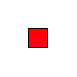
\begin{tikzpicture}\filldraw[draw=black,fill={rgb,255:red,255;green,0;blue,12}](0,0.15)rectangle(0.25,0.4);\end{tikzpicture} Red & Limbic \\ \hline
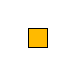
\begin{tikzpicture}\filldraw[draw=black,fill={rgb,255:red,255;green,186;blue,0}](0,0.15)rectangle(0.25,0.4);\end{tikzpicture} Orange & Executive \\ \hline
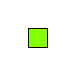
\begin{tikzpicture}\filldraw[draw=black,fill={rgb,255:red,131;green,255;blue,0}](0,0.15)rectangle(0.25,0.4);\end{tikzpicture} Light Green & Rostral-Motor \\ \hline
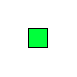
\begin{tikzpicture}\filldraw[draw=black,fill={rgb,255:red,0;green,255;blue,59}](0,0.15)rectangle(0.25,0.4);\end{tikzpicture} Green & Caudal-Motor \\ \hline
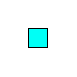
\begin{tikzpicture}\filldraw[draw=black,fill={rgb,255:red,0;green,255;blue,246}](0,0.15)rectangle(0.25,0.4);\end{tikzpicture} Light Blue & Parietal \\ \hline
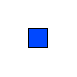
\begin{tikzpicture}\filldraw[draw=black,fill={rgb,255:red,0;green,72;blue,255}](0,0.15)rectangle(0.25,0.4);\end{tikzpicture} Blue & Occipital \\ \hline
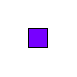
\begin{tikzpicture}\filldraw[draw=black,fill={rgb,255:red,119;green,0;blue,255}](0,0.15)rectangle(0.25,0.4);\end{tikzpicture} Purple & Temporal \\ \hline
\end{tabular}
\caption{Regions Legend}
\label{tab:reglen}
\end{table}
These tracts can be traced to determine their likelihood of reaching specific target regions, such as cortical areas of interest in \reflink{tab:reglen}{Table}. Each voxel within the seed region can be assigned a connectivity value based on the proportion of simulated tracts that successfully reach a given target region, providing a probabilistic measure of connectivity. Once these connectivity values are obtained, the seed region can be segmented, or parcellated, into distinct subregions that are preferentially connected to different targets. This connectivity based parcellation enables a detailed examination of the functional organization of brain regions and their relationship with target areas, contributing valuable insights into both healthy and pathological brain networks.
\begin{figure}[H]
\centering
\includegraphics[width=1\textwidth]{conn}
\caption{Basal Ganglia Parcellation}
\label{fig:conn}
\end{figure}
Different studies have proposed that the ratio of the more commonly obtained T1 and T2 images, can serve as a proxy for myelin. \cite{myelin1} \cite{myelin2} Another study also investigated direct correlations between images \ac{MWF}, T1w/T2w ratio, \ac{FA}, \ac{RD} and \ac{MD}. \cite{myelin3}

\section{Motivation}

The recent studies mentioned in the previous section raise the question, what if some of these \ac{DTI} related images could be synthetized and predicted from simple structural T1 and T2 \ac{MRI} images. This would enable skipping the time and resource consuming process performing \ac{DTI} and potentially even further post processing algorithms like tractography. And it would also have the added benefit of being able to synthetize these less commonly available images from already available historical records.

\section{Objectives}

The goal of this research will be to try to predict \ac{FA} and \ac{MD} from the T1 and T2 images. With the additional goal of predicting relative connectivity. Furthermore, the experiments will include neurologically healthy participants (controls) and participants with Huntington's Disease (patients). This will allow making observations about the influence of neurodegeneration to the stability of the method.

\subsection{Delimitations}

This research will be limited to the Basal Ganglia as the \ac{ROI}, making it feasible for the timeframe of the thesis.

\subsection{Intermediate Goal}

A simpler, intermediate task leading up to the more complex end goals, is a model for the simple segmentation of the Basal Ganglia for the subcortical regions Caudate, Putamen and Accumbens. In order to confirm the feasibility of this project. As this problem is inherently connected to the main goals, as the relative connectivity does obey certain anatomical restrictions, and the subcortical segmentation of the Basal Ganglia is confirmed to be related to the relative connectivity. Thus if this simpler prediction fails, it is almost certain that the complex end goals will fail as well.

%Hospital de Bellvitge provided an excellent dataset of anatomocal \ac{MRI} and \ac{DTI} records of 32 control and 38 Huntington patient records of T1 and T1/T2 \ac{MRI} images with isotropic voxels of 1 millimeter resolution and \ac{DTI} \ac{FA}, \ac{MD} and \ac{RD} images with isotropic voxels of 2 millimeter resolution. Furthermore this dataset also contains the mask for the basal ganglia, which will also be referenced as the \ac{ROI}. Masks for the 7 main cortical regions of the brain, which will also be referenced as the target regions: Limbic, Executive, Rostral-Motor, Caudal-Motor, Parietal, Occipital and Temporal are also included in the dataset. Tractography was performed on the \ac{DTI} images to figure out which parts of the \ac{ROI} are connected to which cortical target, in a similar manner to how it was done in this \citelink{conn}{paper}; where the relative connectivity maps are representing the ratio of the number of streamlines to each cortical target. Furthermore, the raw streamline images are also available, where there are a maximum of 5000 streamlines starting from each voxel in the \ac{ROI}. The subcortical segmentation of the Basal Ganglia is also available, for the Caudate, Putamen and Accumbens on the control records. And lastly \ac{FNIRT} warp fields were also provided for converting the records into normalized space.\par
%Furthermore, for both the \ac{ROI} and cortical targets, the dataset distinguishes between the right and left hemispheres of the brain. Thus there are actually 2 \ac{ROI}s and $2 \cdot 7=14$ target regions.


\chapter{Design}
\section{Preprocessing}

\subsection{Raw Data}
All provided data are in the \ac{NIfTI} format, first these are need to be understood and parsed. This format stores the raw output of the \ac{MRI} record, and additionally an affine transformation matrix which can transform this raw space in order to align them with each other.

\subsubsection{Available Data}
The following data will be preprocessed and read, even if not all of them are going to be used later on it helps providing the largest possible flexibility.

TODO squigly line

\begin{table}[H]
\centering
\begin{tabular}{|l|l|c|c|l|l|}
\hline
\textbf{Data} & \textbf{Shape} & \textbf{Range} & \textbf{Type} & \textbf{Space} & \textbf{Reference} \\ \hline
\ac{dMRI} & (118, 118, 60, 74) & $[0,3000]$ & float & diffusion$_1$ & diffusion \\ \hline
Diffusion \ac{FA} & (118, 118, 60) & $[0,~2]$ & float & diffusion$_2$ & diffusion\_fa \\ \hline
Diffusion \ac{MD} & (118, 118, 60) & $[0,~0.01]$ & float & diffusion$_2$ & diffusion\_md \\ \hline
Diffusion \ac{RD} & (118, 118, 60) & $[0,~0.01]$ & float & diffusion$_2$ & diffusion\_rd \\ \hline
T1 & (208, 256, 256) & $[0,~1000]$ & float & t1$_1$ & t1 \\ \hline
T1/T2 & (208, 256, 256) & $[0,1]$ & float & t1$_2$ & t1t2 \\ \hline
Cortical Targets & (118, 118, 60, 14) & $\{0,1\}$ & bool & diffusion$_1$ & targets \\ \hline
Relative Connectivity & (118, 118, 60, 14) & $[0,1]$ & float & diffusion$_1$ & connectivity \\ \hline
Streamline Image & (118, 118, 60, 14) & $[0,5000]$ & uint & diffusion$_1$ & streamline \\ \hline
\ac{ROI} Mask (Basal Ganglia) & (118, 118, 60, 2) & $\{0,1\}$ & bool & diffusion$_1$ & mask\_basal \& roi \\ \hline
Brain Mask & (208, 256, 256) & $\{0,1\}$ & bool & t1$_1$ & mask\_brain \\ \hline
Basal Ganglia Segmentation & (208, 256, 256) & $[0, 58]$ & uint & t1$_1$ & mask\_basal\_seg \\ \hline
\end{tabular}
\caption{Raw Datapoint}
\label{tab:datas1}
\end{table}

\subsubsection{Registration}
The process of aligning different records into the same native space is called "registration". The provided dataset comes with with 4 different spaces, earlier referenced to as t1$_1$, t1$_2$, diffusion$_1$ and diffusion$_2$. Most of the data are in diffusion$_1$ space, thus it is logical to register the rest into the same space. The registration is done with Dipy TODO REFERENCE bla bla.

\subsubsection{Brain Mask}
The provided dataset did not apply the brain masks for the T1 images out of the box so it can be done with a simple element wise multiplication.

\subsubsection{Native Space}
Transforming two different readings into the same native space requires a bit of math. As \ac{NIfTI} format stores the origin of the data at an arbitrary location in the voxel space. After applying the extracted transformation matrices, the records will line up, but the origin of the voxel space will be at somewhere inside it, instead of at $(0,0,0)$. Meaning that only the first quadrant will be visible of the record, thus the space is also needed to be translated with the negative vector of the transformed space's bounding box's lower end.\par
The translation value can be calculated by calculating the boundaries of the transformed space's bounding box. Get all 8 corners of the voxel space and apply the transformation matrix to all of them. Then get the min-max coordinates along X, Y and Z from the 8 transformed vectors, yielding the lower and upper bounds of the transformed space's bounding box.\par
It is very important to use the same translation value across different raw spaces to properly align them in the native space. For example let $D$ and $T$ denote a diffusion and t1 records and $M_D$ and $M_T$ denote their respective transformation matrices. Let $T_D$ and $T_T$ denote their respective translation values. In order to properly align them we need to apply $A_D = (M_D \cdot {\color{red}T_D})$ matrix and $A_T = (M_T \cdot {\color{red}T_D})$ matrix to $D$ and $T$ respectively, with matching ${\color{red}T_D}$ translation values.\par
The last issue is the missaligned new shapes of the T1 and Diffusion records. This can be simply fixed by truncating the excess along each dimension.

\subsubsection{Uniform Shape}
After aligning the data into the same space per datapoint, it is still very likely that the individual datapoints do not have a uniform shape. This is due to them being in native space, some records will contain a smaller volume brain, some will contain a larger, they will not be the same.\par
Fixing this can be done by figuring out the min-max boundaries along each axis that the brain masks take up in the voxel space. Then the range of the masks along each axis can be calculated from the lower and upper boundaries per datapoint. And then the max range can be selected per axis, across all datapoints, yielding the new uniform shape. Finally, the voxel spaces can be sliced down to the new uniform shape, which can fit all brains of all data points (with some padding for most of them).\par
Note that this fix also greatly improves space efficiency, as it cuts out the unused voxels. This will be beneficial for storage and computational demands of future experiments.
\begin{table}[H]
\centering
\begin{tabular}{|l|l|c|c|}
\hline
\textbf{Data} & \textbf{Shape} & \textbf{Range} & \textbf{Type} \\ \hline
diffusion & (70, 153, 218, 157, 74) & $[0,4096]$ & float16 \\ \hline
t1 & (70, 153, 218, 157, 1) & $[0,947]$ & float16 \\ \hline
roi & (70, 153, 218, 157, 2) & $\{0,1\}$ & bool \\ \hline
targets & (70, 153, 218, 157, 14) & $\{0,1\}$ & bool \\ \hline
connectivity & (70, 153, 218, 157, 14) & $[0,1]$ & float16 \\ \hline
diffusion\_mask & (70, 153, 218, 157, 1) & $\{0,1\}$ & bool \\ \hline
t1\_mask & (70, 153, 218, 157, 1) & $\{0,1\}$ & bool \\ \hline
\end{tabular}
\caption{Uniform Data}
\label{tab:datas2}
\end{table}
Note that the new shapes are all 5 dimensional, where the first dim is for the datapoint index. The next 3 is for the coordinates of the voxels. And the last is for any additional information, like the temporal dimension of the \ac{dMRI} or the target masks or the connectivity labels.

\subsection{Radiomics Features}
Extracting the voxel based radiomic features has two main parameters to tune, the bin width and the kernel width.\par
The two main approaches for binning are absolute discretization and relative discretization. Where in the prior one, a fixed bin width is choosen and in the latter one, a fixed number of bins are chosen and the bin width scales relatively according to the min-max voxel values. \citelink{bin}{This study found that "The absolute discretization consistently provided statistically significantly more reproducible features than the relative discretization."} Relying on this information, the obvious choice to start with is the absolute discretization.\par
The bin width and the kernel width will be tuned in later experiments. And possibly features calculated with different setting will be concatenated and used simultaneously for better results. The used default values will be 25 and 5 for the bin and kernel widths respectively.\par
The following types of radiomic features will be used:
\begin{table}[H]
\centering
\begin{tabular}{|l|c|}
\hline
\textbf{Feature Type} & \textbf{Number of Features} \\ \hline
First Order & 18 \\ \hline
\ac{GLCM} & 23 \\ \hline
\ac{GLSZM} & 16 \\ \hline
\ac{GLRLM} & 16 \\ \hline
\ac{NGTDM} & 5 \\ \hline
\ac{GLDM} & 14 \\ \hline
3D Shape & 17 \\ \hline
\end{tabular}
\caption{Radiomic Feature Types}
\label{tab:radf0}
\end{table}

\subsubsection{Voxel Based}
The following 92 features will be calculated voxel based:
\bgroup
\setlength\LTleft{-1cm}
\setlength\LTright{-1cm}
\begin{longtable}[H]{|l|l|l|}
\nobreakhline
\textbf{First Order} & \textbf{\ac{GLCM}} & \textbf{\ac{GLSZM}} \\ \nobreakhline
Energy & Autocorrelation & SmallAreaEmphasis \\ \nobreakhline
TotalEnergy & JointAverage & LargeAreaEmphasis \\ \nobreakhline
Entropy & ClusterProminence & GrayLevelNonUniformity \\ \nobreakhline
Minimum & ClusterShade & GrayLevelNonUniformityNormalized \\ \nobreakhline
10Percentile & ClusterTendency & SizeZoneNonUniformity \\ \nobreakhline
90Percentile & Contrast & SizeZoneNonUniformityNormalized \\ \nobreakhline
Maximum & Correlation & ZonePercentage \\ \nobreakhline
Mean & DifferenceAverage & GrayLevelVariance \\ \nobreakhline
Median & DifferenceEntropy & ZoneVariance \\ \nobreakhline
InterquartileRange & DifferenceVariance & ZoneEntropy \\ \nobreakhline
Range & JointEnergy & LowGrayLevelZoneEmphasis \\ \nobreakhline
MeanAbsoluteDeviation & JointEntropy & HighGrayLevelZoneEmphasis \\ \nobreakhline
RobustMeanAbsoluteDeviation & Imc1 & SmallAreaLowGrayLevelEmphasis \\ \nobreakhline
RootMeanSquared & Imc2 & SmallAreaHighGrayLevelEmphasis \\ \hline
Skewness & Idm & LargeAreaLowGrayLevelEmphasis \\ \nobreakhline
Kurtosis & MCC & LargeAreaHighGrayLevelEmphasis \\ \nobreakhline
Variance & Idmn &  \\ \nobreakhline
Uniformity & Id &  \\ \nobreakhline
 & Idn &  \\ \nobreakhline
 & InverseVariance &  \\ \nobreakhline
 & MaximumProbability &  \\ \nobreakhline
 & SumEntropy &  \\ \nobreakhline
 & SumSquares &  \\ \hline \hline
\textbf{\ac{GLRLM}} & \textbf{\ac{NGTDM}} & \textbf{\ac{GLDM}} \\ \nobreakhline
ShortRunEmphasis & Coarseness & SmallDependenceEmphasis \\ \nobreakhline
LongRunEmphasis & Contrast & LargeDependenceEmphasis \\ \nobreakhline
GrayLevelNonUniformity & Busyness & GrayLevelNonUniformity \\ \nobreakhline
GrayLevelNonUniformityNormalized & Complexity & DependenceNonUniformity \\ \nobreakhline
RunLengthNonUniformity & Strength & DependenceNonUniformityNormalized \\ \nobreakhline
RunLengthNonUniformityNormalized &  & GrayLevelVariance \\ \nobreakhline
RunPercentage &  & DependenceVariance \\ \nobreakhline
GrayLevelVariance &  & DependenceEntropy \\ \nobreakhline
RunVariance &  & LowGrayLevelEmphasis \\ \nobreakhline
RunEntropy &  & HighGrayLevelEmphasis \\ \nobreakhline
LowGrayLevelRunEmphasis &  & SmallDependenceLowGrayLevelEmphasis \\ \nobreakhline
HighGrayLevelRunEmphasis &  & SmallDependenceHighGrayLevelEmphasis \\ \nobreakhline
ShortRunLowGrayLevelEmphasis &  & LargeDependenceLowGrayLevelEmphasis \\ \nobreakhline
ShortRunHighGrayLevelEmphasis &  & LargeDependenceHighGrayLevelEmphasis \\ \nobreakhline
LongRunLowGrayLevelEmphasis &  &  \\ \nobreakhline
LongRunHighGrayLevelEmphasis &  &  \\ \nobreakhline
\caption{Voxel Based Radiomic Features}
\label{tab:radf1}
\end{longtable}
\egroup

\subsubsubsection{Normalization}


\subsubsection{Non-Voxel Based}

\begin{table}[H]
\centering
\begin{tabular}{|l|}
\hline
\textbf{3D Shape} \\ \hline
MeshVolume \\ \hline
VoxelVolume \\ \hline
SurfaceArea \\ \hline
SurfaceVolumeRatio \\ \hline
Sphericity \\ \hline
Maximum3DDiameter \\ \hline
Maximum2DDiameterSlice \\ \hline
Maximum2DDiameterColumn \\ \hline
Maximum2DDiameterRow \\ \hline
MajorAxisLength \\ \hline
MinorAxisLength \\ \hline
LeastAxisLength \\ \hline
Elongation \\ \hline
Flatness \\ \hline
\end{tabular}
\caption{Shape Based Radiomic Features}
\label{tab:radf2}
\end{table}

\subsection{All Data}

\begin{table}[H]
\centering
\begin{tabular}{|l|l|c|c|}
\hline
\textbf{Data} & \textbf{Shape} & \textbf{Range} & \textbf{Type} \\ \hline
diffusion & (70, 153, 218, 157, 74) & $[0,4096]$ & float16 \\ \hline
t1 & (70, 153, 218, 157, 1) & $[0,947]$ & float16 \\ \hline
roi & (70, 153, 218, 157, 2) & $\{0,1\}$ & bool \\ \hline
targets & (70, 153, 218, 157, 14) & $\{0,1\}$ & bool \\ \hline
connectivity & (70, 153, 218, 157, 14) & $[0,1]$ & float16 \\ \hline
diffusion\_mask & (70, 153, 218, 157, 1) & $\{0,1\}$ & bool \\ \hline
t1\_mask & (70, 153, 218, 157, 1) & $\{0,1\}$ & bool \\ \hline
radiomics\_raw & (70, 153, 218, 157, 92) & $[-363,13979179]$ & float32 \\ \hline
radiomics\_scaled & (70, 153, 218, 157, 92) & $[0,1]$ & float16 \\ \hline
\end{tabular}
\caption{Voxel Data}
\label{tab:datasvox}
\end{table}

\begin{table}[H]
\centering
\begin{tabular}{|l|l|c|c|}
\hline
\textbf{Data} & \textbf{Shape} & \textbf{Range} & \textbf{Type} \\ \hline
radiomics\_brain\_raw & (70, 106, 1) & $[-63,79581700189]$ & float64 \\ \hline
radiomics\_roi\_raw & (70, 106, 2) & $[-70,1078755564]$ & float64 \\ \hline
radiomics\_targets\_raw & (70, 106, 14) & $[-124,4799594982]$ & float64 \\ \hline
radiomics\_brain & (70, 106, 1) & $[0,1]$ & float16 \\ \hline
radiomics\_roi & (70, 106, 2) & $[0,1]$ & float16 \\ \hline
radiomics\_targets & (70, 106, 14) & $[0,1]$ & float16 \\ \hline
\end{tabular}
\caption{Non-Voxel Radiomics Data}
\label{tab:datasrad}
\end{table}

\begin{table}[H]
\centering
\begin{tabular}{|l|l|c|}
\hline
\textbf{Data} & \textbf{Length} & \textbf{Type} \\ \hline
radiomics\_features\_vox & 92 & string \\ \hline
radiomics\_log10\_features\_vox & 57 & string \\ \hline
radiomics\_features & 106 & string \\ \hline
\end{tabular}
\caption{Features Names Data}
\label{tab:datasfea}
\end{table}







\chapter{Experiments}
\label{experiments}

First the initial generic hyper parameters were established for all models, which can be shared between different architectures.
\begin{table}[H]
\centering
\begin{tabular}{|l|l|}
\hline
\textbf{Parameter} & \textbf{Value} \\ \hline
radiomics\_brain\_raw & (70, 106, 1) \\ \hline
\end{tabular}
\caption{Generic Initial Hyperparameters}
\end{table}



\section{Classification FNN}

First the starter hyper parameters were established for the classification \ac{FNN} models.

\subsection{Simple 1}


\chapter{Sustainability}
\section{Environmental Aspect}

\subsection{Developement}

The biggest environmental impact of this project was the required computational power to train the models. Over the entire duration of the project, approximately $5,000$ models were trained.\par
As part of it, the most demanding phase was the exhaustive sequential backward feature selection, which in itself required the training of $3,000$ models. The return value of this computation is close to none, as it only marginally increased model performance. The only real benefit is the model being able to reach the same performance using two thirds of the original features. This is a marginal result, because the omitted features belong to different radiomics feature groups, and the biggest overhead for most feature groups is calculating the voxel-based matrix volume, meaning that if not all features are omitted from a feature group, it only decreases the computational requirements marginally.\par
The $3,000$ models for feature selection were trained on a wide variety of GPUs in a network cluster. These GPUs were H100, P40, RTX3060, RTX3090, RTX2080, multiple T4s (Google Collab's), multiple P100s (Kaggle's). Mining the cluster head's log, reveals that around half of these models were trained on the H100 and the other half on the rest. The H100 was consuming around 300 Watts of power while training with a speed of 5s/epoch and taking 30-60 epochs on average to stop. The H100 consumed between $1500 \cdot 0.3$kW $ \cdot 30 \cdot 5$s $ \div 60 \div 60 = 18.75$kWh on the lower and $2 \cdot 18.75 = 37.5$kWh on the upper end. The other half is harder to estimate due to the many different GPUs used in the cluster, but a crude estimate is $1500 \cdot 0.2$kW $ \cdot 30 \cdot 8$s $ \div 60 \div 60 = 20$kWh on the lower and $2 \cdot 20 = 40$kWh on the upper end. Rounding the sum of them up to $80$kWh and adding an extra $30\%$ overhead for running the rest of the components of the servers/PCs, results in an upper boundary of $104$kWh consumed during the feature selection.\par
The remaining $2,000$ models were trained on the P40 and RTX3060, with the P40 training approximately three fourths of them. Doing the same estimations for the P40 yields $1500 \cdot 0.2$kW $ \cdot 30 \cdot 7$s $ \div 60 \div 60 = 17.5$kWh on the lower and $2 \cdot 17.5 = 35$kWh on the upper end. For the RTX3060, it yields $500 \cdot 0.15$kW $ \cdot 30 \cdot 7$s $ \div 60 \div 60 = 4.375$kWh on the lower and $2 \cdot 4.375 = 8.75$kWh on the upper end. Rounding their sum up to $45$kWh and adding an extra $30\%$ overhead for running the rest of the components of the server, results in an upper boundary of $58.5$kWh consumed during the the rest of the trainings.\par
Feature extraction run on a CPU, with the entire server consuming 200 Watts during the process. The entire duration for the feature extraction run was around 2 weeks. Its total power consumption was $0.2$kW $ \cdot 14$d $ \cdot 24$h $ = 67.2$kWh.\par
In summary, this project had the environmental impact summarized in \reflink{tab:sus1}{Table}, for an average of $0.25$€/kWh for the price of the electricity \cite{kwhprice} and $0.2$kgCO$_{2}$e/kWh for the emission \cite{carbon}:
\begin{table}[H]
\centering
\begin{tabular}{|l|l|l|l|}
\hline
\textbf{Part} & \textbf{Consumption} & \textbf{Price} & \textbf{Emission} \\ \hline
feature selection & $104$kWh & $26$€ & $20.8$kgCO$_{2}$e \\ \hline
rest of the experiments & $58.5$kWh & $14.6$€ & $11.7$kgCO$_{2}$e \\ \hline
feature extraction & $67.2$kWh & $16.8$€ & $13.4$kgCO$_{2}$e \\ \hline
\textbf{Total} ($+10\%$ overhead; rounded up) & $260$kWh & $65$€ & $52$kgCO$_{2}$e \\ \hline
\end{tabular}
\caption{Sustainability: Power Consumptions and CO$_{2}$ Emissions}
\label{tab:sus1}
\end{table}
For reference, this number is a bit less than the average Spanish household's monthly power consumption of $324$kWh. \cite{kwhavg}

\subsection{Production}
\label{sec:susprod}

This project, whether implemented in a production, clinical or research setting, has the potential to significantly enhance sustainability in its respective fields. Acquiring \ac{DTI} data typically requires up to 40 minutes, depending on the specific parameters, whereas obtaining a T1 image takes only about 8 minutes, making data acquisition a considerable time-saving step. Additionally, \ac{DTI} data demands extensive and labor-intensive preprocessing. \textbf{Accelerating clinical or research workflows by a factor of 5} not only saves time but also increases the capacity for data collection or patient processing by the same factor.\par
Synthesizing a single record of relative connectivity or diffusion \ac{FA}/\ac{MD} takes only a few seconds on a GPU, while the radiomic feature extraction takes around 20 minutes. This translates into an approximate energy demand of $200$W $ \cdot (5$s $ \div 60 + 20$m$) \div 60 = 67$Wh for synthetizing a record. It can be argued that the time saved with the data acquisition is lost with the time it takes to extract the radiomic features, but neither the doctor (or MRI operator) and patient need to be present during the computation of the feature extraction. Assuming that an \ac{MRI} machine has a consumption of $25$-$70$kW \cite{kwhmri} and calculating with an average of $50$kW, adds up to a power requirement of $50$kW $ \cdot 40$m $ \div 60 = 33.3$kWh per \ac{DTI} record. Adding up the total energy requirements of T1 data acquisition and record synthesis is $50$kW $ \cdot 8$m $ \div 60 + 67$Wh $ \div 1000 = 6.7$kWh per record. This means that \textbf{this method could be 5 times more sustainable than the traditional approach}, while returning the energy consumption of the development phase in the data acquisition of $260 \div (33.3 - 6.7) = 10$ records, which is naturally a minuscule number when compared to how many \ac{MRI} recordings are routinely acquired in the world.

\section{Economic Aspect}

\subsection{Cost}

The electricity cost during the development phase amounted to $65$€. Approximately half of this cost was covered by colleagues and their networks, who contributed computational resources during the feature selection process. Additional support came from free services provided by Google and Kaggle.\par
Realistically, billing this project would consist of three components: the cost of labor, the price of the server used for development, and the electricity consumed. With the electricity cost already detailed, the server cost and labor are interconnected. The project could have been executed on a less powerful machine, though this would have required more time and more careful focus on software design. Throughout the development, the primary limiting factors were RAM and disk storage. Significant effort was invested in developing efficient data structures and optimizing the memory footprint to address these constraints.\par
In conclusion, the minimum hardware which this project could be feasibly executed on is 32GBs of RAM, Intel Core i5-12600K (or similar), Nvidia RTX3060 (or similar), and $256$GBs of storage. The current cost (new parts ordered from Amazon) of such server (with 'cheap' consumer grade hardware) would be around $300$€ for the GPU, $150$€ for the CPU, $50$€ for the RAM, $25$€ for the SSD, and $150$€ for the motherboard, adding up to $675$€. The main limiting factors in this configuration are the RAM, which was utilized up to $128$GBs during development; and disk storage, which was utilized up to $300$GBs. The extra RAM and storage would cost an additional $200$€ and $25$€ totalling at a new sum of $900$€.\par
The development of this project required approximately $500$ hours of work. Making calculations using the average hourly rate of $19$€ corresponding to a software engineer in Spain \cite{salary}, leads to a total labor cost of $19$€ $ \cdot 500$h $ = 9500$€. Therefore, the total billing for the project would be the one summarized in \reflink{tab:sus2}{Table}:
\begin{table}[H]
\centering
\begin{tabular}{|l|l|l|l|}
\hline
\textbf{Part} & \textbf{Price} \\ \hline
Cumulative Salary & $9500$€ \\ \hline
Server Components & $900$€ \\ \hline
Electricity & $65$€ \\ \hline
\textbf{Total} & $10465$€ \\ \hline
\end{tabular}
\caption{Project Cost Breakdown}
\label{tab:sus2}
\end{table}

\subsection{Return}

This project is by all means a proof of concept, aiming to assess the viability of the proposed approach. More information on the exact conclusions can be found in \reflink{sec:conclusions}{Chapter}, but the potential return value of this project is huge.\par
As stated in the previous \reflink{sec:susprod}{subsection}, this project has the potential to accelerate the clinical and/or research workflows by a factor of 5. The economic implications are applicable for both clinical and research workflows. In the clinical workflow, \textbf{this could increase the number of patients processed by a factor of 5}, with minimal extra cost (especially if compared to the alternative of buying 4 additional \ac{MRI} machines and hiring operators for them). In a research workflow, it would probably have less of an economic impact, but more of a logistical one, as it could simplify the data acquisition, thus \textbf{allowing researchers to have up to 5 times more data acquired} with minimal extra resources invested. But even more importantly, it opens the door of processing past anatomical \ac{MRI} records, as they are much more common than \ac{DTI} records, virtually \textbf{increasing the available data for researchers by several orders of magnitude} (depending on the exact application).

\section{Social Aspect}

\subsection{Inclusivity}
\label{sec:inclusive}

Out of the potential inclusivity aspects, including age, gender, sex, and cultural diversity, it is sex the one that requires most attention, as males and females have slightly different brain structures. \cite{sexbrain} For the control records used, there are 17 male and 15 female ones, which is a relatively even split; for the patient records, there are 25 male and 13 female records, which is relatively unbalanced. This could, in theory, negatively impact the under-represented group if there were truly any differences between the two sexes that mattered from the model’s perspective. However, in this project, and due to the very limited number of records available, it was not an option to discard one third of the patients in order to have the a completely balanced dataset. Moreover, it would need further experimentation so as to determine if this aspect truly impacts the results.\par
This potential difference was overlooked during most of the project’s lifetime, but it should have been included as another constant ratio to be kept during the train/validation/test splitting, which was covered in \reflink{sec:travaltes}{subsection}. Due to limited time for thesis completion and resources, the models were not re-trained with this new rule in mind, and this is something that has been included in the \reflink{sec:improve}{Future Improvements} subsection.\par
The rest of the considerations are less pressing and hard to take into account, like the brain structure of different ethnicities, given that this dataset does not contain any information regarding this aspect. The only other aspect potentially under consideration should be age, but this is partially accounted for as part of the constant symptomatic/asymptomatic ratio, because being symptomatic is closely related to the \ac{CAP} score (covered in \reflink{sec:clinical}{subsection}), which is directly related to age. Thus symptomatic/asymptomatic is indirectly related to age.

\section{Risks}

Environmental, Economic and Social risks are not really applicable to this project, as it is a foundational proof of concept research project.









\chapter{Conclusions}
\label{sec:conclusions}

This foundational project has huge potential thanks to the possible returns and applications of the approach proposed. Due to deployment time and resource limitations, the experiments only focused on the Basal Ganglia, so by no means any of the performance metrics prove that a generalized solution is viable. However the \ac{FA} and \ac{MD} predictions are really promising, and would be interesting to see how would it perform on the entire brain, and not just the \ac{ROI}. On the other hand, the Relative Connectivity predictions are not even nearly precise enough to call them usable, but, admittedly, the labels themselves will inherently contain quite a bit of noise, due to the very sensitive process of extracting the labels with tractography.\par
This project only delved into a tiny fraction of the endless sea of possible preprocessing approaches, and it only experimented with some very basic model architectures. Nevertheless, the viability of this approach and hypothesis is not disproven, but it definitely needs the implementation of some new ideas to make it fully functional.\par

Key conclusions regarding different imaging modalities and spatial normalization primarily stem from the \ac{FA} and Relative Connectivity experiments. The \ac{MD} and Subcortical Segmentation experiments showed only marginal differences across modalities, making it difficult to draw definitive conclusions from these results.\par
In general, experiments conducted in normalized space slightly outperformed those in native space (by 1-2\%). This could be attributed to the removal of some variance in normalized space or reduced misalignment between anatomical \ac{MRI} and \ac{DTI} images.\par
An interesting observation across many experiments was that the T1/T2 modality, despite showing marginally better training performance (by 1-2\%), exhibited more significant overfitting. This resulted in similar validation performance and slightly worse test performance (by 1-2\%) compared to T1. Notably, T1/T2 performed comparably or better with less input data, such as when only a single kernel size of voxel-based features were provided. This suggests that the T1/T2 modality, although not performing as well overall as T1, might harbor untapped potential, particularly in certain conditions.\par
There are alternative explanations for why the results do not fully align with state-of-the-art studies that use the T1/T2 ratio as a myelin proxy. One possible factor is the non-isotropic voxel size of our T2 images, which, when combined with 3D radiomic feature extraction, may introduce noise or bias, particularly affecting the \ac{GLRLM} feature class. This issue could distort feature values due to the skewed run lengths along the affected axis.\par
The neurodegeneration observed in patients with \ac{HD} significantly impacts model performance, likely due to the higher variance in their data. This issue could potentially be mitigated by increasing the dataset size to account for this variability. However, mixing Control and Patient records resulted in only a slight performance decrease, suggesting that combining the two groups lead to more robust models.\par
The inclusion of clinical features exhibited inconsistent results across experiments and modalities. While some configurations led to improved performance in Patient records, these models never outperformed those trained on Control or Control+Patient data, indicating that clinical features may not be a beneficial input in this context.\par
Data augmentation had minimal impact on the native space experiments, likely due to the limited variation introduced by the mild rotations applied during augmentation. More aggressive augmentation could compromise applicability, as it would likely introduce unrealistic variations not typically observed in the raw \ac{MRI} scans.\par
It was also consistently shown in the experiments, that the logarithmic data normalization on the heavily skewed features, did improve performance.\par
Exploring hemisphere-specific datapoints revealed an unexpected finding: the right hemisphere consistently performed better than the left. This pattern can be explained in part by the asymmetrical neurodegeneration in \ac{HD}, where the left hemisphere is affected more severely. Interestingly, this trend was also present in the Control group, which warrants further investigation. Ultimately, combining both hemispheres resulted in models that generalized well, even for the left hemisphere, indicating that training on a mix of hemispheric data may lead to more versatile models.\par

\section{Future Improvements}
\label{sec:improve}

As mentioned in \reflink{sec:seqback}{subsection}, there was a serious oversight during the execution of the exhaustive sequential backwards feature selection. At the time it was believed that the model was performing better on balanced data, due to a bug in the code. Thus, all of these models are performing much worse than the models during the experimentation. The bug was fixed, but due to limited time and resources the feature selection was not executed again.\par
Further investigation of the sex imbalance issue reported in subsection \reflink{sec:inclusive}{subsection} reveals that, with the seed used for the experiments results are not terribly imbalanced for the most part, but there is definitely room for improvement by enforcing a constant ratio. The male/(male+female) ratio for the control record splits is $0.49$/$0.67$/$0.67$ (train/validation/test), while it is $0.62$/$0.5$/$1$ for the patient records.\par
Additionally, one aspect was not investigated thoroughly over the thesis: the kernel size, binning parameters, and feature class relationships during the voxel based feature extraction. For the sake of simplicity, only a unified binning method was used for all kernel sizes and all feature classes. But, logically, the binning parameters could be optimized for each kernel size and feature class. For example, the \ac{GLRLM} feature class could yield fundamentally different features even just by adjusting the bin size a tiny bit at large kernel sizes.\par
The selection of the most efficient kernel size combinations was not investigated thoroughly either. Due to limited resources, the maximum kernel size used was 21, but there was no reason to stop there.\par
Ultimately, and even with the relatively few simple aspects that were taken into consideration during this thesis, the hyperparameter space is gigantic and some compromises had to be made. After investing over 500 hours into this project, the educated guesses for these potential improvements are:
\begin{itemize}
  \item The feature selection should have a marginal improvement on the model performance.
  \item The gender imbalance should not have a measurable impact on the model performance on this scale (with less than 70 available records in total).
  \item The binning parameter optimization for the kernel sizes and feature classes would probably have a big impact on the model performance.
\end{itemize}
And lastly, all experiments should be repeated at least a few times, with different splits and seeds. And the experiments should be evaluated with the means and medians of the model performance indicators, across different runs.\par
Ultimately there are two paths that could be followed in order to pursue this approach further: First, the \ac{FA} and \ac{MD} experiments could be expanded to the entire brain and a generalized model could be developed. The second one would entail the refinement of the Relative Connectivity experiments, as they require overall improvements and the development of new ideas.









%TC:ignore
\printbibliography[heading=bibintoc,title={Sources of Information}]
\appendix

\chapter{Software Design}
The software design was mainly guided by the provided format of the raw data. Which was from a few different sources, as different people were working with different data at the Hospital, and they did not have a unified collection. Thus the following documentation of the software design will be structured going from the raw data, to the preprocessed data, and then the model itself.

\section{Raw Data}

The raw data is scattered amongst many files, are registered in different spaces, does not have masks applied, along with other challenges detailed in \reflink{sec:preproc}{Section}.

\begin{figure}[H]
\centering
\includegraphics[width=0.7\textwidth]{DataRaw}
\caption{Files: Raw}
\end{figure}

The following class diagram documentations are detailed abstractions of the actual source code, as \ac{UML} is not completely Python compliant. Before moving on, the following simple data types are used in the \ac{UML} diagrams:

\begin{figure}[H]
\centering
\includegraphics[width=0.7\textwidth]{ClassDataTypes}
\caption{Class Diagram: Data Types}
\end{figure}

There is one odd one out in this diagram, that being the LayeredArray, which is more than a simple data type or primitive. This class is a simple space efficient data structure of a 4D tensor.\par
Storing some of the data provided can be highly inefficient by storing the raw tensor. Ultimately the design aims to collect the scattered data from multiple files, into clean logical groups, for example all the cortical target masks into a single 4D tensor where the 4th dimension is reserved for the multiple targets. But this poses a greatly inefficient way of storing the data, as each target region only takes up a small portion of the entire space. The idea behind the LayeredArray class, it stores the 4D tensor as a list of 3D tensors, each cropped down to their effective space where there are non-zero voxels. This also requires an additional list of 3D vectors to store each layer's origin, and where to paste it in the original space.\par
This solution offers a very efficient way of storing data for this use case, as the raw storage solution for the cortical targets were around 50MBs, and this cuts it down to 3MBs. This is even more drastic for the relative connectivity, which is more than a simple boolean mask and proportionally takes up even less space of the entire brain; in which's case it was cut down from 110MBs to 0.5MBs, reducing the disk requirement by several magnitudes.\par
The original \ac{NIfTI} format also does a very good job at storing data efficiently, but this solution provides control over the way of storing the data on a much lower level. This is beneficial as the data are stored in numpy format, making it easier to ignore certain data type safety checks, data type conversions, and leaving behind the \ac{NIfTI} format's additional complexity of the orientation, transformation, and many more nuances that are part of the \ac{NIfTI} header.\par
This has the undoubted drawback of not being able to use \ac{FSL} tools natively on our datatypes, such as fsleyes for simply viewing a record. But thanks to the opensource nature of the \ac{FSL} suite, with a few additional lines of code, support can be added for our datatypes (included in \reflink{apx:source}{Appendix}).

\begin{figure}[H]
\centering
\includegraphics[width=0.7\textwidth]{ClassPreprocessing}
\caption{Class Diagram: Preprocessing}
\end{figure}

The class diagram above contains the two classes responsible for the preprocessing of the data. The RecordHandler being the controller itself that handles the high level operations on a collection of records. And the records handling the low level computations on the data itself.

\section{Common Functions}

There are set of static common functions, which give the low level backbone of the entire project. They are grouped into two categories, util and visual. Where the prior one contains everything from simple data type castings, external \ac{FSL} library system calls, to computing radiomics, and more. And the latter one is a collection of functions for visualizing data.

\begin{figure}[H]
\centering
\includegraphics[width=0.7\textwidth]{ClassCommon}
\caption{Class Diagram: Common}
\end{figure}

\section{Preprocessed Data}

Preprocessing the data are composed from the next few high level operations done by the RecordHandler:
\begin{enumerate}
  \item Register some records (not needed for most of them)
  \item Compute all normalized records
  \item Compute the inverse \ac{FNIRT} warp field
  \item Convert native records into our numpy format (apply the affine transformations, merge different sources, etc.)
  \item Compute scaling factors across all native records
  \item Preload native records
  \item Convert normalized records into our numpy format
  \item Compute scaling factors across all normalized records
  \item Preload normalized records
  \item Construct normalized coordinate maps
  \item Warp normalized coordinate maps into native space
  \item Scale and preload coordinate maps
  \item Impute clinical data
\end{enumerate}

After preprocessing, the next set of logical groupings and files are left, split into native and noramlized records:

\begin{figure}[H]
\centering
\includegraphics[width=0.7\textwidth]{DataPreprocessed}
\caption{Files: Preprocessed}
\label{fig:files}
\end{figure}

\section{Data Generator}

As this project focuses on only the voxels inside the Basal Ganglia, means the model on a datapoint level is never going to operate outside of that volume.

\begin{figure}[H]
\centering
\includegraphics[width=0.7\textwidth]{ClassExperimentation}
\caption{Class Diagram: Experimentation}
\end{figure}

The DataGenerator class is responsible for feeding the Model with data, according to the specifications of the experiments. In order to make this more efficient and fast, loading the entire volume of records from disk can be avoided by 'preloading' the \ac{ROI} from each record. This simply put means that all logical grouping and files specified in \reflink{fig:files}{Figure} are preloaded into 1D and 2D tensors, where the first dimension is the flattened voxels of the \ac{ROI} and the second is whatever layers were stored originally in the last dimension of the spatial data (for example the streamlines of the different traget regions).\par
Computing and persisting the preloaded data vastly speeds up the DataGenerator. Although this has the added consequence that the preloaded data yields a pair of tensors instead of a single volume, as there is differentiation between the left and right hemispere datapoints. And the voxel count in the two hemispheres are not symmetrical, thus the hemisphere differentiation can not be stored as an extra dimension. A design decision was made to store the left and right hemisphere data in separate files.\par
The properties of the DataGenerator provided in its constructor defines the type and format of the generated data.

\begin{longtable}[H]{|L{3cm}|L{3cm}|L{10cm}|}
\hline
\textbf{Value} & \textbf{Type} & \textbf{Description} \\ \hline
path & string & path of the data \\ \hline
seed & int & random seed for the train/val/test splits \\ \hline
split & float & train/all ratio \\ \hline
test\_split & float & test/(test+validation) ratio \\ \hline
control & boolean & include control records \\ \hline
huntington & boolean & include huntington records \\ \hline
left & boolean & include left hemisphere datapoints \\ \hline
right & boolean & include right hemisphere datapoints \\ \hline
threshold & FLOAT & if not None it thresholds the labels by setting the values under the provided threshold to zero; if 0 it re-one-hot encodes the labels (sets the maximum label to 1 and the rest to 0) \\ \hline
binarize & boolean & if thresholded and True, it also sets the labels above the threshold to 1 (and the rest to 0) \\ \hline
not\_connected & boolean & if thresholded and True, it appends an additional 'not connected' label, which complements the sum of the labels per voxel to 1 \\ \hline
single & INT & if not None it only returns the label with the provided index \\ \hline
features & List$<$string$>$ & used non-voxel based radiomics features (emptylist means all) \\ \hline
features\_vox & List$<$string$>$ & used voxel based radiomics features (emptylist means all) \\ \hline
radiomics: List$<$Radiomics$>$ & space: string & space of non-voxel based radiomic features \newline (native/normalized) \\ \cline{2-3}
 & image: string & input image of non-voxel based radiomic features \newline (t1/t1t2) \\ \cline{2-3}
 & features: List$<$string$>$ & list of binning settings of the features \newline (b25, b50, b10r... etc.) \\ \cline{2-3}
 & files: List$<$string$>$ & list of region mask settings of the features \newline (targets/roi/brain) \\ \hline
space & string & space of voxel based radiomic features \newline (native/normalized) \\ \hline
radiomics\_vox: List$<$ & image: string & input image of voxel based radiomic features \newline (t1/t1t2) \\ \cline{2-3}
{   }RadiomicsVox \newline$>$ & features: List$<$string$>$ & list of binning and kernel settings of the features \newline (k5\_b25, k9\_b50, k7\_b10r... etc.) \\ \hline
rad\_vox\_norm & string & use normalization, or only min-max scaling on the voxel based radiomic features (norm/scale) \\ \hline
inps & List$<$string$>$ & additional voxel inputs (t1/t1t2/diffusion/diffusion\_fa/ diffusion\_md/diffusion\_rd) \\ \hline
features\_clin & List$<$string$>$ & additional clinical data inputs (empty array means all) \\ \hline
outp & string & output (connectivity/streamline/basal\_seg/ diffusion\_fa/diffusion\_md/diffusion\_rd) \\ \hline
balance\_data & boolean & enables data balancing \\ \hline
balance\_bins & int & number of bins used for continuous data when balancing \\ \hline
balance\_ratio & float & ratio of the resampling of the difference between each bin and the max bin when balancing (where 0 is unbalanced and 1 is perfectly balanced) \\ \hline
exclude & List$<$string$>$ & can manually add missing groups of records to exclude (t1t2/normalized/basal\_seg/diffusion\_fa) \\ \hline
reinclude & List$<$string$>$ & can manually re-include (append) missing groups of records to the train split (t1t2/normalized/basal\_seg/diffusion\_fa) \\ \hline
debug & boolean & only returns 1/1/1 records for train/val/test when True \\ \hline
augment & List$<$string$>$ & list of record suffixes, used to include augmented records in the training split; for example the suffix '\_5\_0\_0' is used for the rotation augmentation of 5, 0 and 0 degrees on the X, Y and Z axis (naturally these records needs to be computed before using here) \\ \hline
\caption{Data Generator Properties}
\end{longtable}








\chapter{Software Implementation}
\label{app:impl}

Detailing the entire implementation of the project is beyond the scope of this report. But some solutions contain non self explanatory ideas and are worthy of detailed explanations. For more details please refer to the source code.

\section{Interpolation}

One crucial detail of applying transformations to the records, is the type of interpolation used. For some images like T1 the standard trilinear interpolation makes sense, as the values inbetween voxels should be continuous. However for some other images like binary masks, the interpolation should be nearest neighbour, as the edge of the mask cant be interpreted as a fraction. And most importantly the relative connectivity and streamline images should also be interpolated with nearest neighbour, preserving their characteristics like their summed total being 1 per voxel for the relative connectivity. In theory the streamline image could be computed with trilinear interpolation, after which the relative connectivity could be computed from the interpolated streamlines. But this would degrade the streamline images due to their unbalanced nature of having a few voxels with high number of streamlines relative to the entire voxel space, effectively eroding the boundaries of the high intensity volumes.\par
In practice this meant using 0th and 1st order spline interpolations, which are numerically the same as nearest neighbour and trilinear interpolations.

\section{Multithreading}

As most of the preprocessing could not be easily offloaded to the GPU (without re-implementing major libraries such as 'pyradiomics' with GPU support), it was crucial to implement multithreading to save time.\par
The most straight forward way of doing so was to split the load on a record level, and process multiple records paralel. Testing revealed an interesting property of the feature extraction, which is the RAM IO operation bottleneck of the process. Extracting voxel based features happen in a 'voxel batch', which seemed to only increase the RAM usage of the process beyond a certain point, but not the speed. After days of tweaking and running tests, it was concluded that computing the \ac{GLCM} feature class is RAM IO operation heavy. Meaning that increasing voxel batch size or the number of threads (computing different records in parallel) will not increase the performance past a certain point, as the threads are waiting on RAM IO operations regardless.\par
The optimal settings with the used Intel Core i5-12600K CPU and 128GBs of 3200MT/s RAM, is to use 7 threads, out of which 5 are dedicated for computing the \ac{GLCM} feature class and the rest 2 are for computing other feature classes, with a voxel batch size of 1000.\par
Trying to increase performance this point by increasing the voxel batch size, or the number of threads only resulted in the same, or worse overall performance due to the computational overhead of splitting and merging the work between more threads, and using a lot more RAM.

\section{Warp Pre-Computing}
\label{app:imp-pre}

As mentioned in \reflink{sec:eval}{subsection}, computing the evaluation metrics both in native and normalized space can be done by reconstucting the spatial records from the predicted datapoints and warping them to native/normalized space, and then re-extracting the datapoints from the warped records. However this would be computationally very expensive to do so every time when calculating the evaluation metrics.\par
The solution is to pre-compute index arrays, by assigning unique indexes to the voxels of the records, warping the records, and mapping the \ac{ROI}'s flattened voxels' unique indexes between the (warped and non-warped) record pairs into an index array which can be used to quickly and efficiently convert the voxels of the \ac{ROI} between native and normalized spaces.

\begin{figure}[H]
\centering
\includegraphics[width=0.3\textwidth]{warp_precompute}
\caption{Index Array Mapping}
\end{figure}

\section{Data Normalization}
\label{app:imp-norm}

As noted in \reflink{sec:norm}{subsection}, determining which voxel-based radiomic features require log scaling for distribution normalization is handled programmatically. This process involves loading each feature across all records and analyzing their distribution both before and after log scaling.\par
Initially, the feature is min-max scaled, and the distribution of non-zero voxels is calculated using $100$ bins (bin size $0.01$). Excluding zero values masks the background, which would distort the distribution. However, this exclusion should have been done with the provided brain masks, which would have been more appropriate since zeros could naturally occur in the features. This oversight, while suboptimal, does not significantly affect the results, as non-background zero counts are negligible. And the only consequence is a potential false negative artifacts (failing to apply normalization where needed), which does not degrade the raw data by inappropriately normalizing features.\par
Next, the logarithm is applied to the feature prior to min-max scaling, and the distribution is recalculated using the same $100$ bin approach. The criteria for selecting normalized features are based on observing an increased standard deviation and a reduced count of voxels in the largest bin after normalization. This ensures that features with 'flattened' and 'stretched' distributions are selected for normalization.








\titlespacing*{\chapter}{0pt}{-70pt}{30pt}
\chapter{Additional Figures}
%\vspace{-2in}

\begin{figure}[H]
\centering
\includegraphics[width=0.9\textwidth]{rad_gldm_small_scale_16}
\includegraphics[width=0.9\textwidth]{rad_gldm_small_scale_32}
\includegraphics[width=0.9\textwidth]{rad_gldm_small_norm_16}
\caption{Slice: GLDM Small Dependence High Gray Level Emphasis}
\label{fig:gls}
\end{figure}

\begin{figure}[H]
\centering
\includegraphics[width=0.9\textwidth]{rad_ngtdm_busyness_scale_16}
\includegraphics[width=0.9\textwidth]{rad_ngtdm_busyness_scale_32}
\includegraphics[width=0.9\textwidth]{rad_ngtdm_busyness_norm_16}
\caption{Slice: NGTDM Busyness}
\label{fig:ngb}
\end{figure}

\begin{figure}[H]
\centering
\includegraphics[width=0.7\textwidth]{subcortical_curve}
\caption{Training Curve: Subcortical}
\label{fig:curve-sub}
\end{figure}

\begin{figure}[H]
\centering
\includegraphics[width=0.9\textwidth]{subcortical_train_o}
\includegraphics[width=0.9\textwidth]{subcortical_train_p}
\caption{Train Predictions: Subcortical}
\label{fig:pred-tra-sub}
\end{figure}

\begin{figure}[H]
\centering
\includegraphics[width=0.9\textwidth]{subcortical_val_o}
\includegraphics[width=0.9\textwidth]{subcortical_val_p}
\caption{Validation Predictions: Subcortical}
\label{fig:pred-val-sub}
\end{figure}

\begin{figure}[H]
\centering
\includegraphics[width=0.9\textwidth]{subcortical_test_o}
\includegraphics[width=0.9\textwidth]{subcortical_test_p}
\caption{Test Predictions: Subcortical}
\label{fig:pred-tes-sub}
\end{figure}

\begin{figure}[H]
\centering
\includegraphics[width=0.7\textwidth]{md_curve}
\caption{Training Curve: Mean Diffusivity}
\label{fig:curve-md}
\end{figure}

\begin{figure}[H]
\centering
\includegraphics[width=0.9\textwidth]{md_train_o}
\includegraphics[width=0.9\textwidth]{md_train_p}
\caption{Train Predictions: Mean Diffusivity}
\label{fig:pred-tra-md}
\end{figure}

\begin{figure}[H]
\centering
\includegraphics[width=0.9\textwidth]{md_val_o}
\includegraphics[width=0.9\textwidth]{md_val_p}
\caption{Validation Predictions: Mean Diffusivity}
\label{fig:pred-val-md}
\end{figure}

\begin{figure}[H]
\centering
\includegraphics[width=0.9\textwidth]{md_test_o}
\includegraphics[width=0.9\textwidth]{md_test_p}
\caption{Test Predictions: Mean Diffusivity}
\label{fig:pred-tes-md}
\end{figure}

\begin{figure}[H]
\centering
\includegraphics[width=0.7\textwidth]{fa_curve}
\caption{Training Curve: Diffusion Fractional Anisotropy}
\label{fig:curve-fa}
\end{figure}

\begin{figure}[H]
\centering
\includegraphics[width=0.9\textwidth]{fa_train_o}
\includegraphics[width=0.9\textwidth]{fa_train_p}
\caption{Train Predictions: Diffusion Fractional Anisotropy}
\label{fig:pred-tra-fa}
\end{figure}

\begin{figure}[H]
\centering
\includegraphics[width=0.9\textwidth]{fa_val_o}
\includegraphics[width=0.9\textwidth]{fa_val_p}
\caption{Validation Predictions: Diffusion Fractional Anisotropy}
\label{fig:pred-val-fa}
\end{figure}

\begin{figure}[H]
\centering
\includegraphics[width=0.9\textwidth]{fa_test_o}
\includegraphics[width=0.9\textwidth]{fa_test_p}
\caption{Test Predictions: Diffusion Fractional Anisotropy}
\label{fig:pred-tes-fa}
\end{figure}

\begin{figure}[H]
\centering
\includegraphics[width=0.7\textwidth]{con_curve}
\caption{Training Curve: Relative Connectivity}
\label{fig:curve-con}
\end{figure}

\begin{figure}[H]
\centering
\includegraphics[width=0.9\textwidth]{con_train_o}
\includegraphics[width=0.9\textwidth]{con_train_p}
\caption{Train Predictions: Relative Connectivity}
\label{fig:pred-tra-con}
\end{figure}

\begin{figure}[H]
\centering
\includegraphics[width=0.9\textwidth]{con_val_o}
\includegraphics[width=0.9\textwidth]{con_val_p}
\caption{Validation Predictions: Relative Connectivity}
\label{fig:pred-val-con}
\end{figure}

\begin{figure}[H]
\centering
\includegraphics[width=0.9\textwidth]{con_test_o}
\includegraphics[width=0.9\textwidth]{con_test_p}
\caption{Test Predictions: Relative Connectivity}
\label{fig:pred-tes-con}
\end{figure}



\titlespacing*{\chapter}{0pt}{-10pt}{30pt}
\chapter{Additional Tables}
\bgroup
\setlength\LTleft{-1cm}
\setlength\LTright{-1cm}
\begin{longtable}[H]{|l|l|l|}
\nobreakhline
\textbf{First Order} & \textbf{\ac{GLCM}} & \textbf{\ac{GLSZM}} \\ \nobreakhline
Energy & Autocorrelation & SmallAreaEmphasis \\ \nobreakhline
TotalEnergy & JointAverage & LargeAreaEmphasis \\ \nobreakhline
Entropy & ClusterProminence & GrayLevelNonUniformity \\ \nobreakhline
Minimum & ClusterShade & GrayLevelNonUniformityNormalized \\ \nobreakhline
10Percentile & ClusterTendency & SizeZoneNonUniformity \\ \nobreakhline
90Percentile & Contrast & SizeZoneNonUniformityNormalized \\ \nobreakhline
Maximum & Correlation & ZonePercentage \\ \nobreakhline
Mean & DifferenceAverage & GrayLevelVariance \\ \nobreakhline
Median & DifferenceEntropy & ZoneVariance \\ \nobreakhline
InterquartileRange & DifferenceVariance & ZoneEntropy \\ \nobreakhline
Range & JointEnergy & LowGrayLevelZoneEmphasis \\ \nobreakhline
MeanAbsoluteDeviation & JointEntropy & HighGrayLevelZoneEmphasis \\ \nobreakhline
RobustMeanAbsoluteDeviation & Imc1 & SmallAreaLowGrayLevelEmphasis \\ \nobreakhline
RootMeanSquared & Imc2 & SmallAreaHighGrayLevelEmphasis \\ \hline
Skewness & Idm & LargeAreaLowGrayLevelEmphasis \\ \nobreakhline
Kurtosis & MCC & LargeAreaHighGrayLevelEmphasis \\ \nobreakhline
Variance & Idmn &  \\ \nobreakhline
Uniformity & Id &  \\ \nobreakhline
 & Idn &  \\ \nobreakhline
 & InverseVariance &  \\ \nobreakhline
 & MaximumProbability &  \\ \nobreakhline
 & SumEntropy &  \\ \nobreakhline
 & SumSquares &  \\ \hline \hline
\textbf{\ac{GLRLM}} & \textbf{\ac{NGTDM}} & \textbf{\ac{GLDM}} \\ \nobreakhline
ShortRunEmphasis & Coarseness & SmallDependenceEmphasis \\ \nobreakhline
LongRunEmphasis & Contrast & LargeDependenceEmphasis \\ \nobreakhline
GrayLevelNonUniformity & Busyness & GrayLevelNonUniformity \\ \nobreakhline
GrayLevelNonUniformityNormalized & Complexity & DependenceNonUniformity \\ \nobreakhline
RunLengthNonUniformity & Strength & DependenceNonUniformityNormalized \\ \nobreakhline
RunLengthNonUniformityNormalized &  & GrayLevelVariance \\ \nobreakhline
RunPercentage &  & DependenceVariance \\ \nobreakhline
GrayLevelVariance &  & DependenceEntropy \\ \nobreakhline
RunVariance &  & LowGrayLevelEmphasis \\ \nobreakhline
RunEntropy &  & HighGrayLevelEmphasis \\ \nobreakhline
LowGrayLevelRunEmphasis &  & SmallDependenceLowGrayLevelEmphasis \\ \nobreakhline
HighGrayLevelRunEmphasis &  & SmallDependenceHighGrayLevelEmphasis \\ \nobreakhline
ShortRunLowGrayLevelEmphasis &  & LargeDependenceLowGrayLevelEmphasis \\ \nobreakhline
ShortRunHighGrayLevelEmphasis &  & LargeDependenceHighGrayLevelEmphasis \\ \nobreakhline
LongRunLowGrayLevelEmphasis &  &  \\ \nobreakhline
LongRunHighGrayLevelEmphasis &  &  \\ \nobreakhline
\caption{Voxel Based Radiomic Features}
\label{tab:radf1}
\end{longtable}
\egroup

\begin{table}[H]
\centering
\begin{tabular}{|l|}
\hline
\textbf{3D Shape} \\ \hline
MeshVolume \\ \hline
VoxelVolume \\ \hline
SurfaceArea \\ \hline
SurfaceVolumeRatio \\ \hline
Sphericity \\ \hline
Maximum3DDiameter \\ \hline
Maximum2DDiameterSlice \\ \hline
Maximum2DDiameterColumn \\ \hline
Maximum2DDiameterRow \\ \hline
MajorAxisLength \\ \hline
MinorAxisLength \\ \hline
LeastAxisLength \\ \hline
Elongation \\ \hline
Flatness \\ \hline
\end{tabular}
\caption{Shape Based Radiomic Features}
\label{tab:radf2}
\end{table}


\chapter{Source Code}
\dirtree{%
.1 source.
.2 data.
.3 models.
.3 native.
.4 preloaded.
.4 preprocessed.
.4 raw.
.3 normalized.
.4 preloaded.
.4 preprocessed.
.4 raw.
.3 preprocessed.
.3 raw.
.2 logs.
.2 fsleyes.
.2 distributed.
.1 experiments.
.2 subcortical.
.2 diffusion\_md.
.3 native-t1.
.3 native-t1t2.
.3 normalized-t1.
.3 normalized-t1t2.
.3 architecture.
.2 diffusion\_fa.
.3 native-t1.
.3 native-t1t2.
.3 normalized-t1.
.3 normalized-t1t2.
.3 architecture.
.2 connection.
.3 native-t1.
.3 native-t1t2.
.3 normalized-t1.
.3 normalized-t1t2.
.3 architecture.
.2 streamline.
.2 misc.
.1 report.
.2 progress.
.2 project.
}


% \texttt{ }\par
% \noindent \textbf{android-camera-imu} the source code of the auxiliary camera-imu app\par
% \texttt{ }\par
% \noindent \textbf{diagrams} exported UML diagrams\par
% \texttt{ }\par
% \noindent \textbf{doc} some of the \path{.tex} files\par
% \noindent \textbf{appendices} appendix \path{.tex} files\par
% \noindent \textbf{chapters} chapter \path{.tex} files\par
% \noindent \textbf{images} figures\par

%================== EXAMPLES ==================
% \includepdf[pages=1,pagecommand={\chapter[Project Description]{} \label{app:projdesc}},linktodoc=true]{Appendix_A/ProjectDescription.pdf}
% \includepdf[pages=2-]{Appendix_A/ProjectDescription.pdf}
% \chapter{Machine Vision Class Descriptions} \label{app:CVclassdesc}
% \input{appendices/classdesccpp}
% \includepdf[pages=1,pagecommand={\chapter[User Manual]{} \label{app:manual}},linktodoc=true]{Appendix_D/UserManual.pdf}
% \includepdf[pages=2-]{Appendix_D/UserManual.pdf}
% \chapter{Unit Test Descriptions and Test Results} \label{app:CVunittestdesc}
% \input{appendices/unittestdesccpp}
% \chapter{Integration Test Results} \label{app:CVintegrationtestdesc}
% \input{appendices/integrationtestdesccpp}
% \includepdf[pages=1,pagecommand={\chapter[Process Report]{} \label{app:procrep}},linktodoc=true]{Appendix_G/ProcessReport.pdf}
% \includepdf[pages=2-]{Appendix_G/ProcessReport.pdf}
%==============================================

%TC:endignore
\end{document}